\begin{frame}[c]
  \frametitle{Context}
%rajouter le titre (version courte) dans toute les slides
\begin{center}
  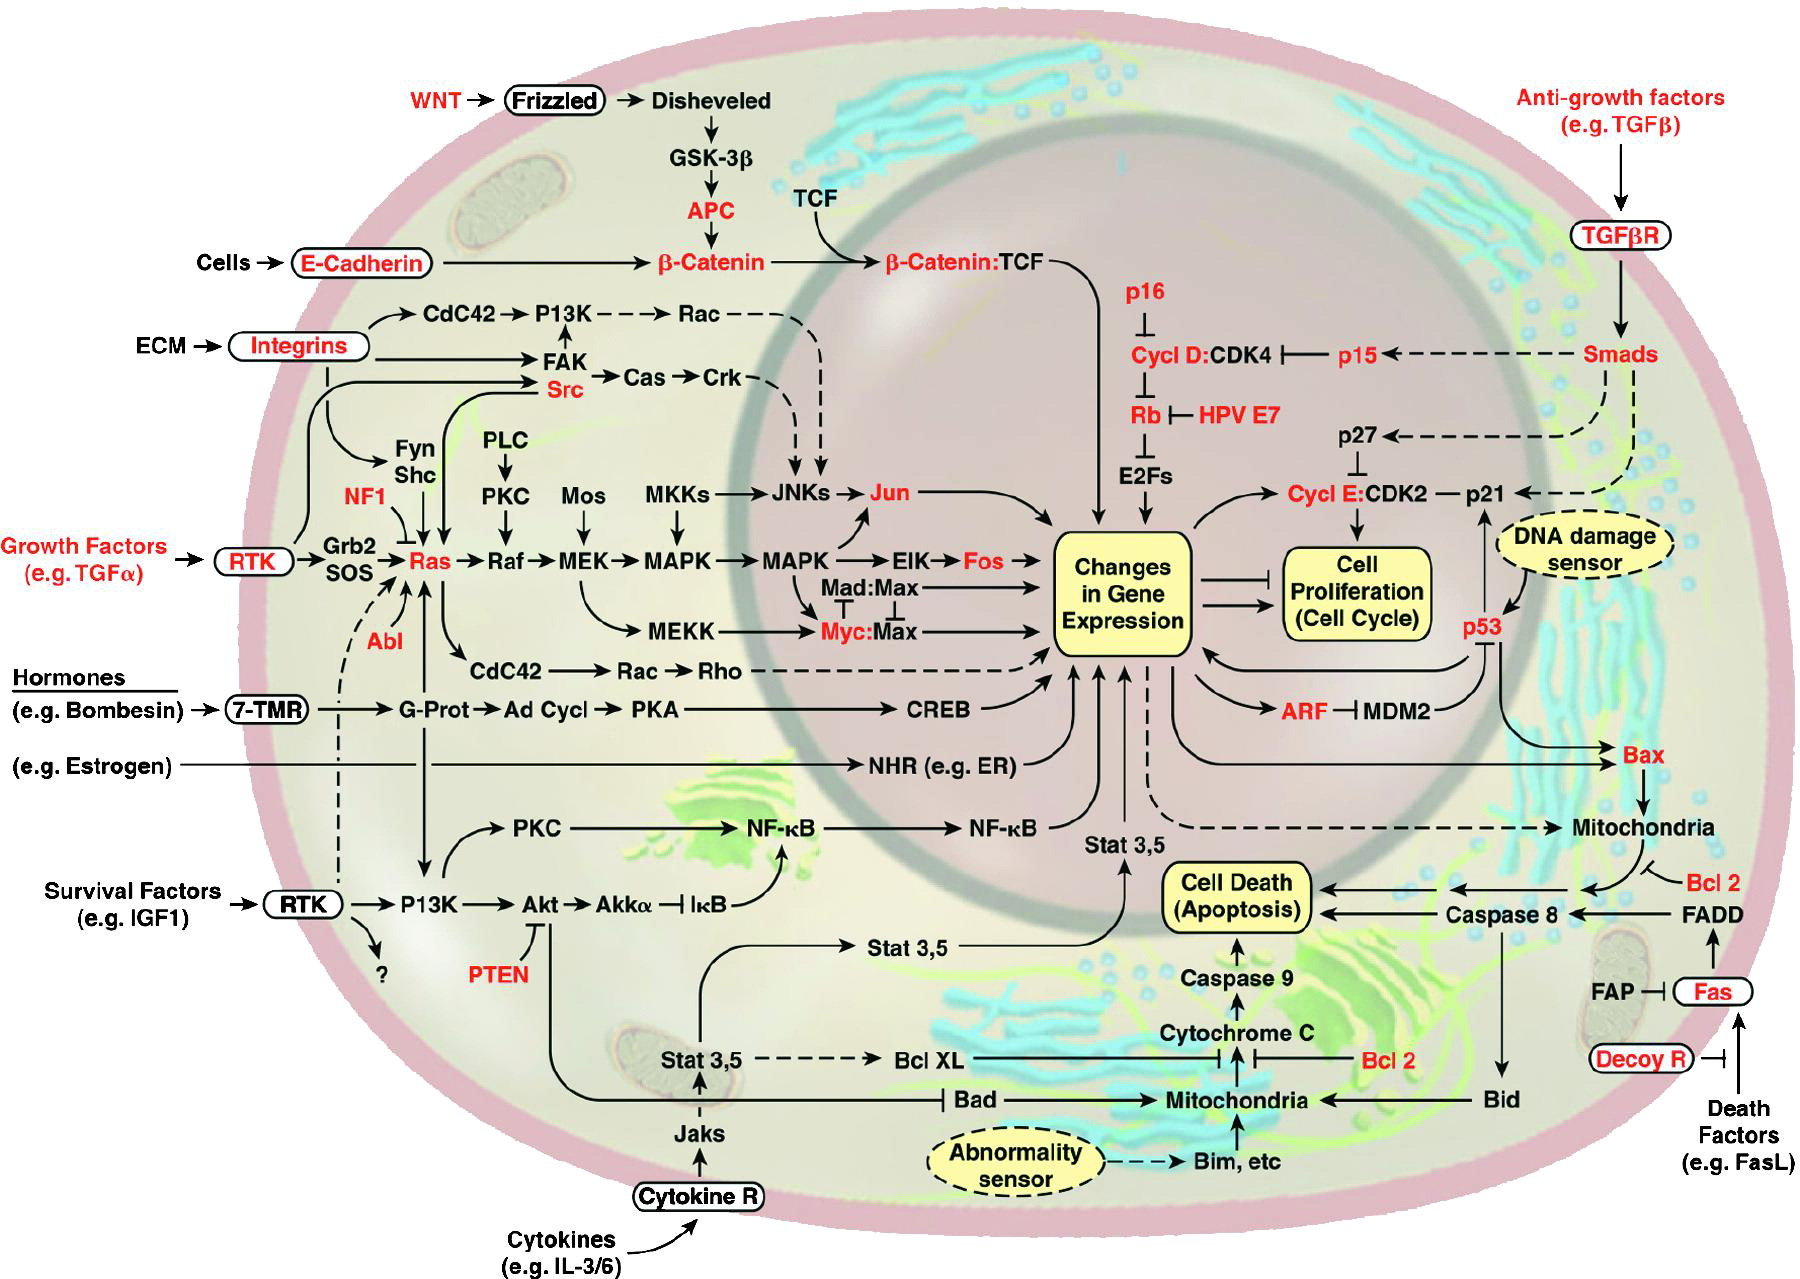
\includegraphics[scale=0.12]{images/cellule-description.jpeg}
\end{center}
\begin{center}
{\tiny \color{darkgreen}[\citelui]}
\end{center}

%\tcite{Wikipédia}

\begin{itemize}
\item Cellular processes $\Longrightarrow$ networks of biological interactions.
\item Nodes (biological components), edges (interactions).
\end{itemize}

%Cellular processes are driven by networks of biological reactions. Cells rely on the tight coordination of these pathways to achieve proper functioning.
%With the help of signaling pathway, a cell senses changes in its environnement or internal state. This information is then passed on via cascades of biochemical 
%reactions to the appropriate mechanisms which respond by modifying the metabolic and transcriptiona activities. this in turn modifies the behavior of the cell.

%Consequently, the dynamics of biopathways play a crucial role in determinig cellular functions.

%Examples: circadian rhythm, the apoptosis pathway inducing programmed cell death, cell differentiation.

%\textcolor{couleurtheme}{$\Rightarrow$} \fbox{\tval{\large The need of comprehension of biological systems}} \textcolor{couleurtheme}{$\Leftarrow$}


%\textcolor{couleurtheme}{$\Rightarrow$} \fbox{\tval{\large Allow efficient translation from Process Hitting to BRN}} \textcolor{couleurtheme}{$\Leftarrow$}

\end{frame}

\begin{frame}[c]
 \frametitle{Motivation}
  %\pause
 %figure illustrative
 \begin{tikzpicture}[auto]

\path[use as bounding box] (-0.7,-2) rectangle (3,3);

%le noeud pour les connaissances de la littérature, générales
\node[align=center] (gk) at (2,3) {\begin{tabular}{|c|}
\hline
 General knowledge  \\
 \hline
 Literature  \\
  \hline
 Hypotheses   \\
  \hline
\end{tabular}};

%\pause

%les noeud pour le réseau biologique
\node[qgre] (a) at (1,1.5) {a};
\node[mod] (i) at (2.3,1) {i};
\node[qgre] (b) at (1,0.5) {b};
\node[qgre] (c) at (3,1) {c};


\path
 (a) edge[act] node[center]{$p_1$\footnotesize ?} (i)
 (b) edge[inh] node[below]{\color{red} $p_2$\footnotesize ?} (i)
 (i) edge[st]  (c);

 %\pause

\node (deco) at (2,-0.1) {Times series data};
\node[align=center] (tsd) at (2,-1) {\begin{tabular}{|c|c|c|c|}
\hline
 Genes  & 1h & ... & 24h  \\
 \hline
 Gene $1$  &   & ...  &    \\
  \hline
  Gene $2$  &   & ...  &    \\
  \hline
\end{tabular}};


\onslide<2->{

\node (d1) at (5,1) {};
\node (d2) at (7.5,1) {};

\node (d3) at (4.5,-1.5) {};
\node (d4) at (4.5,3.5) {};


\draw[->,line width=6pt, color=lightgray] (d1) -- (d2) node[above=10pt,midway]{\textcolor{black}{\textbf{Algebraic Modelling}}};
}

\onslide<2->{
%le modèle en process hitting
\node[scale=0.4] (phmodel) at (10,1) {\begin{tikzpicture} \exphHM
                           \end{tikzpicture}};
}

\end{tikzpicture}

\onslide<2->{
Formal inference of the parameters of Biological Networks:

  \begin{itemize}
   \item Avoid critical behaviors.
  \end{itemize}

}

\end{frame}
                   

